\begin{center}

\includegraphics[width=0.4\textwidth]{content/3/chapter4/images/44.png}\\
Cippi is ready for the race
\end{center}

With C++20, we get new and improved attributes such as [[nodiscard("reason")]], [[likely]], [[unlikely]], and [[no\_unique\_address]]. In particular, [[nodiscard("reason")]] can be used to explicitly express the intent of our interface.


\begin{tcolorbox}[colback=blue!5!white,colframe=blue!75!black,title={Attributes}]
Attributes allow the programmer to express additional constraints on the source code or give the compiler additional optimization possibilities. You can use attributes for types, variables, functions, names, and code blocks. When you use more than one attribute, you can apply each one after the other (func1) or all together in one attribute, separated by commas (func2):

\noindent
Use of attributes
\begin{lstlisting}[style=styleCXX]
[[attribute1]] [[attribute2]] [[attribute3]]
int func1();

[[attribute1, attribute2, attribute3]]
int func2();
\end{lstlisting}

Attributes can be implementation-defined language extensions or standard attributes, such as the following list of attributes C++11 - C++17 already have.

\begin{itemize}
\item 
{}[[noreturn]] (C++11): indicates that the function does not return

\item 
{}[[carries\_dependency]] (C++11): indicates a dependency chain in \href{https://en.cppreference.com/w/cpp/atomic/memory_order#Release-Consume_ordering}{release-consume ordering}

\item 
{}[[deprecated]] (C++14): indicates that you should not use a name

\item 
{}[[fallthrough]] (C++17): indicates that a fallthrough in a case branch is intentional

\item 
{}[[maybe\_unused]] (C++17): suppresses compiler warning about used names
\end{itemize}
\end{tcolorbox}


\subsubsubsection{4.8.1\hspace{0.2cm} [[nodiscard("reason")]]}

C++17 introduced the new attribute [[nodiscard]] without a reason. C++20 added the possibility to add a message to the attribute.

\noindent
Discarding objects and error codes
\begin{lstlisting}[style=styleCXX]
// withoutNodiscard.cpp

#include <utility>

struct MyType {

	MyType(int, bool) {}

};

template <typename T, typename ... Args>
T* create(Args&& ... args) {
	return new T(std::forward<Args>(args)...);
}

enum class ErrorCode {
	Okay,
	Warning,
	Critical,
	Fatal
};

ErrorCode errorProneFunction() { return ErrorCode::Fatal; }

int main() {

	int* val = create<int>(5);
	delete val;
	
	create<int>(5);
	
	errorProneFunction();
	
	MyType(5, true);

}
\end{lstlisting}

Thanks to perfect forwarding and parameter packs, the factory function create (line 11) can call any constructor and return a heap-allocated object.

The program has many issues. First, line 30 has a memory leak, because the int created on the heap is never deleted. Second, the error code of the function errorProneFunction (line 32) is not checked. Lastly, the constructor call MyType(5, true) (line 34) creates a temporary, which is created and immediately destroyed. This is at least a waste of resources. Now, [[nodiscard]] comes into play.

[[nodiscard]] can be used in a function declaration, enumeration declaration, or class declaration. If you discard the return value from a function declared as [[nodiscard]], the compiler should issue a warning. The same holds for a function returning by copy an enumeration or a class declared as [[nodiscard]]. If you still want to ignore the return value, you can cast it to void.

Let us see what this means. In the following example, I use the C++17 syntax of the attribute [[nodiscard]].

\noindent
Use of the attribute [[nodiscard]] in C++17
\begin{lstlisting}[style=styleCXX]
// nodiscard.cpp

#include <utility>

struct MyType {

	MyType(int, bool) {}

};

template <typename T, typename ... Args>
[[nodiscard]]
T* create(Args&& ... args){
	return new T(std::forward<Args>(args)...);
}

enum class [[nodiscard]] ErrorCode {
	Okay,
	Warning,
	Critical,
	Fatal
};

ErrorCode errorProneFunction() { return ErrorCode::Fatal; }

int main() {

	int* val = create<int>(5);
	delete val;
	
	create<int>(5);
	
	errorProneFunction();
	
	MyType(5, true);

}
\end{lstlisting}

The factory function create (line 13) and the enum ErrorCode (line 17) are declared as [[nodiscard]]. 
Consequently, the calls in lines 31 and 33 create warnings.

\begin{center}
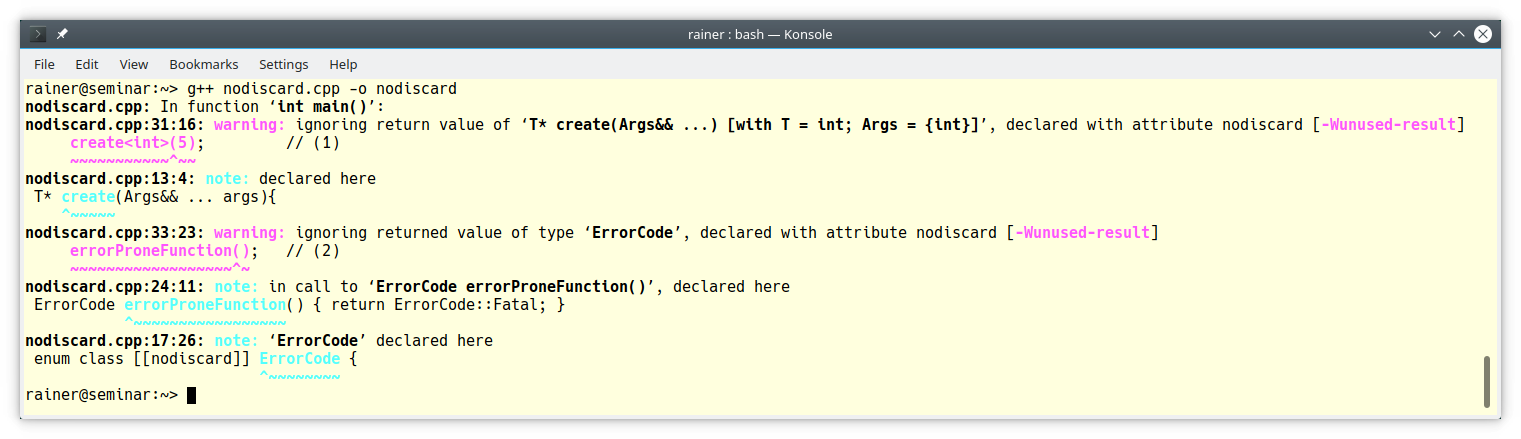
\includegraphics[width=0.6\textwidth]{content/3/chapter4/images/45.png}\\
A C++17 compiler complains about a discarded object and a discarded error code
\end{center}

Way better, but the program still has a few issues. [[nodiscard]] cannot be used for functions such as a constructor returning nothing. Therefore, the temporary MyType(5, true) (line 35) is still created without a warning. Second, the error messages are too general. As a user of the functions, I want to have a reason why discarding the result is an issue.

Both issues can be solved with C++20. Constructors can be declared as [[nodiscard]], and the warning can have additional information.

\noindent
Use of the attribute [[nodiscard]] in C++20
\begin{lstlisting}[style=styleCXX]
// nodiscardString.cpp

#include <utility>

struct MyType {

	[[nodiscard("Implicit destroying of temporary MyInt.")]] MyType(int, bool) {}
	
};

template <typename T, typename ... Args>
[[nodiscard("You have a memory leak.")]]
T* create(Args&& ... args){
	return new T(std::forward<Args>(args)...);
}

enum class [[nodiscard("Don't ignore the error code.")]] ErrorCode {
	Okay,
	Warning,
	Critical,
	Fatal
};
 
ErrorCode errorProneFunction() { return ErrorCode::Fatal; }

int main() {

	int* val = create<int>(5);
	delete val;
	
	create<int>(5);
	
	errorProneFunction();
	
	MyType(5, true);

}
\end{lstlisting}

Now, the user of the functions gets specific messages. Here is the output of the Microsoft compiler.

\begin{center}
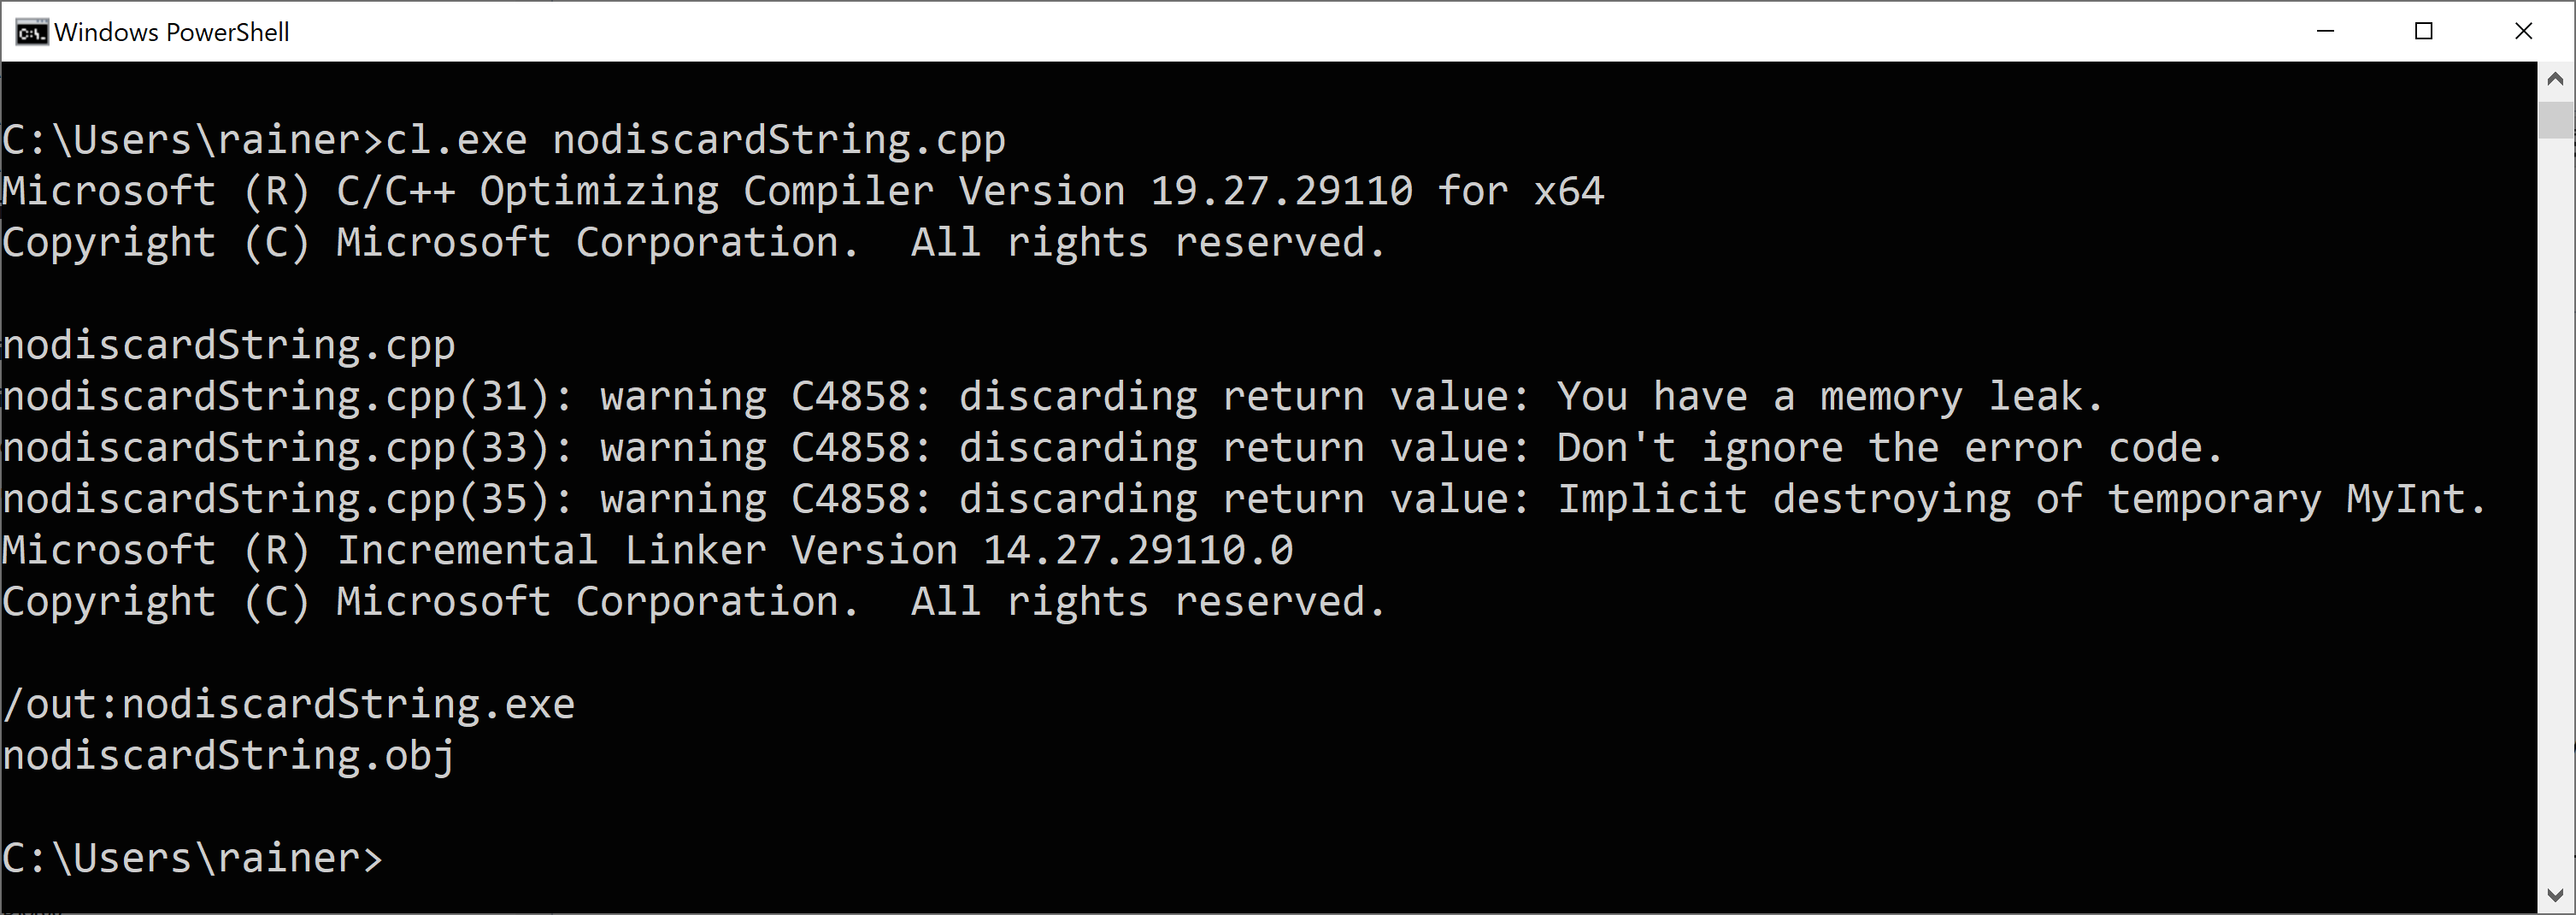
\includegraphics[width=0.6\textwidth]{content/3/chapter4/images/46.png}\\
A C++20 compiler complains about discarded objects and error codes
\end{center}

\begin{tcolorbox}[colback=red!5!white,colframe=red!75!black,title={The issue with std::async}]
Many existing functions in C++ could benefit from the [[nodiscard]] attribute. An ideal candidate is the function std::async. When you don’t use the return value of std::asnyc, what you intended as an asynchronous std::async call implicitly becomes synchronous. What should have run in a separate thread behaves instead as a blocking function call. Read more about the counterintuitive behavior of std::async in my post \href{https://www.modernescpp.com/index.php/the-special-futures}{“The Special Futures”}.

While studying the [[nodiscard]] syntax on \href{https://en.cppreference.com/w/cpp/language/attributes/nodiscard}{cppreference.com/nodiscard}, I noticed that the declarations of \href{https://en.cppreference.com/w/cpp/thread/async}{std::async} changed with C++20. Here is one:

\noindent
std::async uses in C++20 the attribute [[nodiscard]]
\begin{lstlisting}[style=styleCXX]
template<class Function, class... Args>
[[nodiscard]]
std::future<std::invoke_result_t<std::decay_t<Function>,
								 std::decay_t<Args>...>>
	async( Function&& f, Args&&... args );
\end{lstlisting}

The return-type of promise std::async, is declared as [[nodiscard]] in C++20.
	
\end{tcolorbox}

The next two attributes [[likely]] and [[unlikely]] are about optimization.

\subsubsubsection{4.8.2\hspace{0.2cm} [[likely]] and [[unlikely]]}

Proposal \href{http://www.open-std.org/jtc1/sc22/wg21/docs/papers/2018/p0479r5.html}{P0479R5} for the attributes [[likely]] and [[unlikely]] is the shortest proposal I know of. To give you an idea, this is the interesting note to the proposal. “The use of the likely attribute is intended to allow implementations to optimize for the case where paths of execution including it are arbitrarily more likely than any alternative path of execution that does not include such an attribute on a statement or label. The use of the unlikely attribute is intended to allow implementations to optimize for the case where paths of execution including it are arbitrarily more unlikely than any alternative path of execution that does not include such an attribute on a statement or label. A path of execution includes a label if and only if it contains a jump to that label. Excessive usage of either of these attributes is liable to result in performance degradation.” In summary, both attributes allow for giving the optimizer a hint regarding the path of execution expected to be more or less likely.

\noindent
Give the optimizer a hint with [[likely]]
\begin{lstlisting}[style=styleCXX]
for(size_t i=0; i < v.size(); ++i){
	if (v[i] < 0) [[likely]] sum -= sqrt(-v[i]);
	else sum += sqrt(v[i]);
}
\end{lstlisting}

The story of optimization goes on with the new attribute [[no\_unique\_address]]. This time the optimization addresses space instead of execution time.

\subsubsubsection{4.8.3\hspace{0.2cm} [[no\_unique\_address]]}

[[no\_unique\_address]] expresses that this data member of a class need not have an address distinct from all other non-static data members of its class. Consequently, if the member has an empty type, the compiler can optimize it to occupy no memory.

The following program exemplifies the usage of the new attribute.

\noindent
Use of the attribute [[no\_unique\_address]]
\begin{lstlisting}[style=styleCXX]
// uniqueAddress.cpp

#include <iostream>

struct Empty {};

struct NoUniqueAddress {
	int d{};
	[[no_unique_address]] Empty e{};
};

struct UniqueAddress {
	int d{};
	Empty e{};
};

int main() {

	std::cout << '\n';
	
	std::cout << std::boolalpha;
	
	std::cout << "sizeof(int) == sizeof(NoUniqueAddress): "
			  << (sizeof(int) == sizeof(NoUniqueAddress)) << '\n';
	
	std::cout << "sizeof(int) == sizeof(UniqueAddress): "
			  << (sizeof(int) == sizeof(UniqueAddress)) << '\n';
	
	std::cout << '\n';
	
	NoUniqueAddress NoUnique;
	
	std::cout << "&NoUnique.d: " << &NoUnique.d << '\n';
	std::cout << "&NoUnique.e: " << &NoUnique.e << '\n';
	
	std::cout << '\n';
	
	UniqueAddress unique;
	
	std::cout << "&unique.d: " << &unique.d << '\n';
	std::cout << "&unique.e: " << &unique.e << '\n';
	
	std::cout << '\n';

}
\end{lstlisting}

The class NoUniqueAddress has a size equal to int (line 7), but not the class UniqueAddress (line 12). The members d and e of UniqueAddress (lines 40 and 41) have different addresses but not the members of the class UniqueAddress (lines 33 and 34).

\begin{tcblisting}{commandshell={}}
sizeof(int) == sizeof(NoUniqueAddress): true
sizeof(int) == sizeof(UniqueAddress): false

&NoUnique.d: 0x7fff44f8fd0c
&NoUnique.d: 0x7fff44f8fd0c

&unique.d: 0x7fff44f8fd04
&unique.d: 0x7fff44f8fd08
\end{tcblisting}

\begin{center}
Use of the class NoUniqueAddress and UniqueAddress
\end{center}


\begin{tcolorbox}[colback=mygreen!5!white,colframe=mygreen!75!black,title={Distilled Information}]
\begin{itemize}
\item 
C++20 supports a few new attributes. [[nodiscard("reason")]] can be used in various contexts to check if the return value of a function is ignored.

\item 
[[likely]] and [[unlikely]] allows the programmer to give the compiler a hint which code path is more likely to be executed
\item 
Thanks to the attribute [[no\_unique\_address]], data members of a class can have the same address.
\end{itemize}
\end{tcolorbox}


















